\chapter{Logica Fuzzy}\label{fuzzy-set}\index{logica fuzzy}
La logica fuzzy è una logica in cui si può attribuire a ciascuna proposizione un grado di verità compreso tra 0 e 1.

Con grado di verità o valore di appartenenza si intende \emph{quanto è vera} una proprietà: questa può essere, oltre che vera (= a valore 1) o falsa (= a valore 0) come nella logica bivalente, anche pari a valori intermedi.

Formalmente, un insieme fuzzy è una coppia $(U,m)$ dove $U$ è un insieme e $m\colon U \rightarrow [0,1]$. Per ogni $x \in U$, il valore $m(x)$ è chiamato il \emph{grado di appartenenza} di $x$ ad $(U,m)$. Per un insieme finito $U=\{x_1,\dots,x_n\}$, l'insieme fuzzy $(U,m)$ è spesso denotato con $\{m(x_1)/x_1,\dots,m(x_n)/x_n\}$.

Per le scienze cognitive, la logica fuzzy può essere vista come un modello matematico per trattare fenomeni linguistici al fine di creare rappresentazioni della realtà più accurate. L’utilizzo di queste logiche porta benefici sia per la semplicità che per la flessibilità: si possono gestire problemi con dati imprecisi e incompleti, si possono modellare funzioni non lineari di complessità arbitraria.

La teoria degli insiemi fuzzy, introdotta nel 1965 dal prof. Lofti Zadeh\index{Zadeh, Lofti}\footnote{Lotfi Asker Zadeh (Baku, 4 febbraio 1921) è un matematico, ingegnere e ricercatore azero naturalizzato statunitense. È noto soprattutto per i suoi lavori che segnano la nascita della teoria degli insiemi fuzzy nel 1965 (nota in italiano anche come teoria degli insiemi sfocati) e la teoria della logica fuzzy nel 1973.}, fu un cambio di prospettiva rispetto alla teoria classica degli insiemi, che sono raramente adatti a descrivere \emph{matematicamente} problemi \emph{umanistici}. Ad esempio, il problema di descrivere la temperatura di una stanza con gli insiemi bivalenti classici è rappresentato nella figura \ref{fig:bivalent-sets}.\index{logica bivalente}

\begin{figure}[hbt]
  \centering
  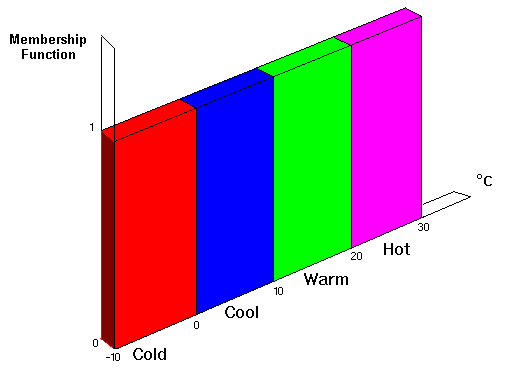
\includegraphics[width=0.7\textwidth]{img/fuzzy-bivalent_temp.png}
  \caption{Rappresentazione della temperatura con insiemi bivalenti}
  \label{fig:bivalent-sets}
\end{figure}

Come si può notare, la più evidente limitazione è che gli insiemi bivalenti sono \emph{mutuamente esclusivi}. Non è possibile infatti avere un membro che appartiene contemporaneamente a due insiemi (\SI{15}{\celsius} appartiene solo all’insieme ``warm''). Soprattutto, nel mondo ``reale'' è poco accurato il fatto che passando da \SI{19}{\celsius} a \SI{20}{\celsius} si passi istantaneamente da ``warm'' a ``hot''.

Il fenomeno naturale può essere meglio descritto dagli insiemi fuzzy. La figura \ref{fig:fuzzy-sets} mostra come questi insiemi possono quantificare l’informazione in modo naturale.

\begin{figure}[hbt]
  \centering
  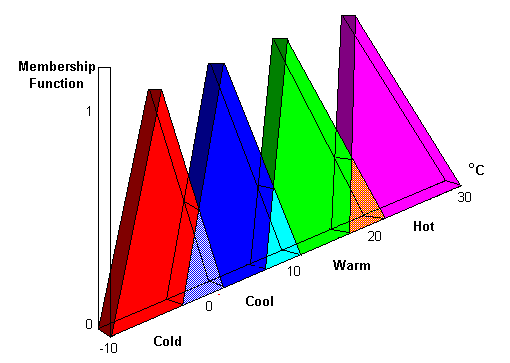
\includegraphics[width=0.7\textwidth]{img/fuzzy-fuzzy_temp.png}
  \caption{Rappresentazione della temperatura con insiemi fuzzy}
  \label{fig:fuzzy-sets}
\end{figure}

\section{Operazioni sugli insiemi fuzzy}
\subsection{Definizioni}
Definiamo $U$ l'\emph{universo} del discorso, ovvero il range di tutti i possibili valori di input per un sistema fuzzy. Dato un $x \in U$, $x$ è ``non appartenente'' all'insieme fuzzy $(A,m)$ se $m(x) = 0$, $x$ è ``totalmente incluso'' se $m(x) = 1$, e ``membro fuzzy'' se $0 < m(x) < 1$.

La funzione $m$ è chiamata ``funzione di appartenenza'' all'insieme fuzzy $(A, m)$. L'insieme $\{x\in U\mid m(x)>0\}$ è chiamato ``supporto'' di $(A,m)$, ovvero l’insieme di tutti i punti dell’universo del discorso $U$ tali che la loro funzione di appartenenza $m$ ad $A$ è diversa da zero. L'insieme $\{x\in A\mid m(x)=1\}$ è chiamato ``kernel'' e rappresenta tutti i punti totalmente inclusi nell'insieme. L'insieme $\{x\in A\mid m(x)=0.5\}$ è chiamato ``punto di crossover'' e rappresenta tutti i punti dell'insieme con funzione di appartenenza $m(x)=0.5$. Un insieme il cui supporto è costituito da un unico punto kernel viene definito ``singleton fuzzy''.

\subsection{Operazioni}

\begin{figure}[hbt]
\centering
\subfloat[][\emph{Unione fuzzy}.]
   {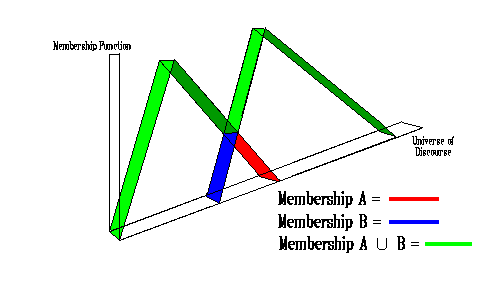
\includegraphics[width=.45\textwidth]{img/fuzzy-union.png}} \quad
\subfloat[][\emph{Intersezione fuzzy}.]
   {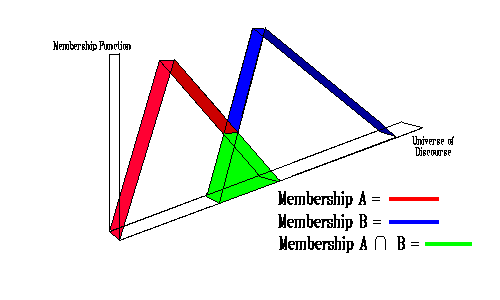
\includegraphics[width=.45\textwidth]{img/fuzzy-intersec.png}} \\
\subfloat[][\emph{Complemento fuzzy}.]
   {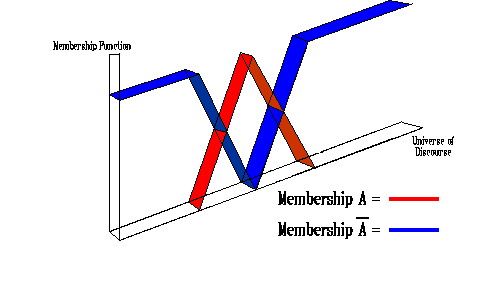
\includegraphics[width=.45\textwidth]{img/fuzzy-comp.png}} \quad
\caption{Rappresentazione grafica delle operazioni sugli insiemi fuzzy}
\label{fig:operazioni}
\end{figure}

\paragraph{Unione}\index{unione fuzzy}
Dati due insiemi fuzzy $A$ e $B$ tali che $A,B \in U$, e $x$ un elemento nell'universo $U$, l'unione è definita come il massimo delle due individuali funzioni di appartenenza: $m_{A \cup B} (x) = \max (m_A (x), m_B (x)) $.

\paragraph{Intersezione}\index{intersezione fuzzy}
Dati due insiemi fuzzy $A$ e $B$ tali che $A,B \in U$, e $x$ un elemento nell'universo $U$, l'unione è definita come il minimo delle due individuali funzioni di appartenenza: $m_{A \cap B} (x) = \min (m_A (x), m_B (x)) $.

\paragraph{Complemento}\index{complemento fuzzy}
Dato un insieme fuzzy $A$ tale che $A \in U$, e $x$ un elemento nell'universo $U$, il complemento dell'insieme fuzzy è definito come $m_A (x) = 1-m_A (x2)$.